%%%%%%%%%%%%%%%%%%%%%%%%%%%%%%%%%%%%%%%%%
% Short Sectioned Assignment
% LaTeX Template
% Version 1.0 (5/5/12)
%
% This template has been downloaded from:
% http://www.LaTeXTemplates.com
%
% Original author:
% Frits Wenneker (http://www.howtotex.com)
%
% License:
% CC BY-NC-SA 3.0 (http://creativecommons.org/licenses/by-nc-sa/3.0/)
%
%%%%%%%%%%%%%%%%%%%%%%%%%%%%%%%%%%%%%%%%%

%----------------------------------------------------------------------------------------
%	PACKAGES AND OTHER DOCUMENT CONFIGURATIONS
%----------------------------------------------------------------------------------------

\documentclass[paper=a4, fontsize=11pt]{scrartcl} % A4 paper and 11pt font size

\usepackage{listings}
\usepackage{color}

\definecolor{dkgreen}{rgb}{0,0.6,0}
\definecolor{gray}{rgb}{0.5,0.5,0.5}
\definecolor{mauve}{rgb}{0.58,0,0.82}

\lstset{frame=tb,
language=Java,
aboveskip=3mm,
belowskip=3mm,
showstringspaces=false,
columns=flexible,
basicstyle={\small\ttfamily},
numbers=none,
numberstyle=\tiny\color{gray},
keywordstyle=\color{blue},
commentstyle=\color{dkgreen},
stringstyle=\color{mauve},
breaklines=true,
breakatwhitespace=true,
tabsize=3
}

\usepackage[T1]{fontenc} % Use 8-bit encoding that has 256 glyphs
\usepackage[utf8]{inputenc}
\usepackage[spanish]{babel} % English language/hyphenation
\usepackage{amsmath,amsfonts,amsthm} % Math packages
% \usepackage{breakcites}
\usepackage{sectsty} % Allows customizing section commands
\allsectionsfont{\centering \normalfont\scshape} % Make all sections centered, the default font and small caps
\usepackage{algorithm}
\usepackage{url}
\usepackage[noend]{algpseudocode}
\makeatletter
\usepackage{graphicx}

\usepackage{fancyhdr} % Custom headers and footers
\pagestyle{fancyplain} % Makes all pages in the document conform to the custom headers and footers
\fancyhead{} % No page header - if you want one, create it in the same way as the footers below
\fancyfoot[L]{} % Empty left footer
\fancyfoot[C]{} % Empty center footer
\fancyfoot[R]{\thepage} % Page numbering for right footer
\renewcommand{\headrulewidth}{0pt} % Remove header underlines
\renewcommand{\footrulewidth}{0pt} % Remove footer underlines
\setlength{\headheight}{13.6pt} % Customize the height of the header
% Reinsert missing \algbackskip
\def\algbackskip{\hskip-\ALG@thistlm}
\renewcommand*{\ALG@name}{Algoritmo}
% \makeatother
\decimalpoint
\numberwithin{equation}{section} % Number equations within sections (i.e. 1.1, 1.2, 2.1, 2.2 instead of 1, 2, 3, 4)
\numberwithin{figure}{section} % Number figures within sections (i.e. 1.1, 1.2, 2.1, 2.2 instead of 1, 2, 3, 4)
\numberwithin{table}{section} % Number tables within sections (i.e. 1.1, 1.2, 2.1, 2.2 instead of 1, 2, 3, 4)

\setlength\parindent{0pt} % Removes all indentation from paragraphs - comment this line for an assignment with lots of text

%----------------------------------------------------------------------------------------
%	TITLE SECTION
%----------------------------------------------------------------------------------------

\newcommand{\horrule}[1]{\rule{\linewidth}{#1}} % Create horizontal rule command with 1 argument of height

\title{	
\normalfont \normalsize 
\textsc{Universidad Nacional de San Agustín, Escuela de Ingenieria de Sistemas} \\ [25pt] % Your university, school and/or department name(s)
\horrule{0.5pt} \\[0.4cm] % Thin top horizontal rule
\huge ADA - Lab 02 \\ % The assignment title
\horrule{2pt} \\[0.5cm] % Thick bottom horizontal rule
}

\author{Fernando Enrique Araoz Morales - 20173373} % Your name

\date{\normalsize\today} % Today's date or a custom date

\begin{document}

\maketitle % Print the title

%----------------------------------------------------------------------------------------
%	PROBLEM 1
%----------------------------------------------------------------------------------------

\section{Introducción}\label{sec:introducción}

En el presente documento se presenta un análisis del tiempo de ejecución del algoritmo Bubble Sort,
con el fin de demostrar el crecimiento exponencial de su tiempo de ejecución.

\section{Implementación}\label{sec:implementación}

La implementacion del algoritmo es la misma provista en la carpeta compartida de Google Drive.


\begin{lstlisting}

    public class BubleSort implements IAlgorithm {

        private int length;

        BubleSort(int length) {
            this.length = length;
        }

        @Override
        public String description() {
            return "Bubble Sort Problem";
        }

        @Override
        public boolean run() {
            // Creates a random array
            int[] data = new int[length];
            for (int i = 0; i < length; i++) {
                data[i] = (int) (Math.random() * 10000);
            }
            System.out.print(length + "i terminado. ");

            // explosive bubble sort
            for (int i = 0; i < length - 1; i++) {
                for (int j = 1; j < length; j++) {
                    if (data[j - 1] > data[j]) {
                        int temp = data[j - 1];
                        data[j - 1] = data[j];
                        data[j] = temp;
                    }
                }
            }
            System.out.print("Orden terminado. ");

            // how to validate??
            for (int i = 1; i < length; i++) {
                if (data[i - 1] > data[i]) return false;
            }
            return true;
        }

    }

\end{lstlisting}

Para facilitar la creacion de datos, el tamaño del array de enteros es dinámico, mediante la
incorporación de un atributo length.


La siguiente clase se encarga de ejecutar el algoritmo con diferente numero de elementos, y
escribe los datos revelantes en un archivo data.csv. Estos datos se describen con mayor detalle
en una sección posterior.

\begin{lstlisting}

    import java.io.FileWriter;
    import java.io.IOException;

    public class BubbleSortDataWriter {

        private String getData(int iteration) {
            long startTime = System.currentTimeMillis();
            boolean result = new BubleSort(iteration).run();
            long endTime = System.currentTimeMillis();
            System.out.println("(" + (endTime - startTime) + "ms)");

            return iteration + ", " + startTime + ", " + endTime + ", " +
            (endTime - startTime) + ", " + result + "\n";
        }

        public void writeData(int iterations, int multiplier, int sum) throws IOException {
            FileWriter fout = null;
            try {
                String writeData;

                fout = new FileWriter("./data.csv");
                fout.write("number_of_elements, start_time, end_time, duration, result\n");
                for (int i = 1; i <= iterations; ++i) {
                    writeData = getData(i * multiplier + sum);
                    fout.write(writeData);
                }

            } catch (IOException e) {
                System.err.println("Error al abrir el archivo para escritura.\n" + e.getMessage());
                e.printStackTrace();
            } finally {
                if (fout != null) {
                    fout.close();
                }
            }
        }

    }

\end{lstlisting}

    Los parámetros multiplier y sum del método writeData se usan para controlar la cantidad de
    elementos a ordenar, e iterations es la cantidad de iteraciones a realizar y escribir en
    el archivo data.csv

\section{Tiempos de ejecución}\label{sec:tiempos-de-ejecución}

    El algoritomo se ejecutó en diferentes intervalos con diferentes cantidades de datos,
    para poder tener la mayor cantidad de información usando la menor cantidad de tiempo.

    En primer lugar, se ejecuto el algoritmo 8000 veces, con desde 1 elemento hasta 8000 elementos,
    aumentando 1 elemento en cada iteración.

    El siguiente segmento realizó iteraciones desde los 8000 elementos hasta los 50000 elementos,
    incrementado en intervalos de 1000 elementos por iteración.

    Luego, iniciando en los 50000 elementos se ejecuto el algoritmo en intervalos de 10000 elementos
    hasta alcanzar los 100000 elementos.

    Finalmente, en intervalos de 50000 elementos se alcanzó la cifra de 400000 elementos.

    Los resultados de estas pruebas se encuentran ilustradas en el suguiente gráfico:

\begin{figure}
    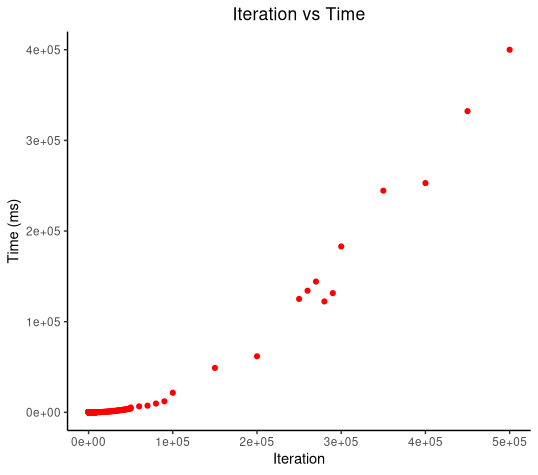
\includegraphics[width=\linewidth]{Rplot.png}
    \caption{Incremento del tiempo de ejecución de Bubble Sort.}
\end{figure}

    Los tiempos de ejecución alcanzan los 400000ms para el caso con 500000 elementos.

\section{Conclusión}\label{sec:conclusión}

    Al observar el gráfico mostrado, podemos apreciar el tiempo de ejecución exponencial
    de este algoritmo, y con ello comprender la importancia del análisis y diseño de algoritmos.
    A través de este, podemos reducir drásticamente el tiempo de ejecución de un algoritmo,
    mejorando su eficiencia masivamente.

%------------------------------------------------

\end{document}